\documentclass[UTF8]{ctexart}
\usepackage{amsmath, amssymb}
\usepackage{enumitem}
\usepackage{tasks}
\usepackage{graphicx}
\usepackage[a4paper, margin=0.6in]{geometry}
\usepackage{amsmath}
\usepackage{amssymb}
\usepackage{tikz}
\usepackage{amsmath}
\usepackage{amssymb}
\usepackage{ulem}  % 用于可能的下划线等,这里用于“最深层循环中的语句”等强调(若需要)

\begin{document}
	
	\section{数据结构}
	
	在分析一个程序的时间复杂性时,有以下两条规则:
	\begin{enumerate}
		\item 加法规则:\( T(n) = T_1(n) + T_2(n) = O(f(n)) + O(g(n)) = O(\max(f(n), g(n))) \)
		\item 乘法规则:\( T(n) = T_1(n) \times T_2(n) = O(f(n)) \times O(g(n)) = O(f(n) \times g(n)) \)
	\end{enumerate}
	
	常见的渐近时间复杂度为  
	\[ O(1) < O(\log_2 n) < O(n) < O(n\log_2 n) < O(n^2) < O(n^3) < O(2^n) < O(n!) < O(n^n) \]
	
	一个语句的频度是指该语句在算法中被重复执行的次数。算法中所有语句的频度之和记为 \( T(n) \),它是该算法问题规模 \( n \) 的函数,时间复杂度主要分析 \( T(n) \) 的数量级。算法中基本运算(\underline{最深层循环中的语句})的频度与 \( T(n) \) 同数量级,因此通常将算法中基本运算的执行次数的数量级作为该算法的时间复杂度\(^{\circ}\)。于是,算法的时间复杂度记为  
	\[ T(n) = O(f(n)) \]  
	
	式中,\( O \) 的含义是 \( T(n) \) 的数量级,其严格的数学定义是:若 \( T(n) \) 和 \( f(n) \) 是定义在正整数集合上的两个函数,则存在正常数 \( C \) 和 \( n_0 \),使得当 \( n \geq n_0 \) 时,都满足 \( 0 \leq T(n) \leq C f(n) \)。
	
	
	算法的空间复杂度 \( S(n) \) 定义为该算法所需的存储空间,它是问题规模 \( n \) 的函数,记为  
	\[ S(n) = O(g(n)) \]  
	
	
	一个程序在执行时除需要存储空间来存放本身所用的指令、常数、变量和输入数据外,还需要一些对数据进行操作的工作单元和存储一些为实现计算所需信息的辅助空间。若输入数据所占空间只取决于问题本身,和算法无关,则只需分析除输入和程序之外的额外空间。例如,若算法中新建了几个与输入数据规模 \( n \) 相同的辅助数组,则空间复杂度为 \( O(n) \)。
	
	算法原地工作是指算法所需的辅助空间为常量,即 \( O(1) \)。
	
	
	\subsubsection{循环主体中的变量参与循环条件的判断}
	
	在用于递推实现的算法中,首先找出基本运算的执行次数 \( x \) 与问题规模 \( n \) 之间的关系式,解得 \( x = f(n) \),\( f(n) \) 的最高次幂为 \( k \),则算法的时间复杂度为 \( O(n^k) \)。
	
	
	\subsubsection{循环主体中的变量与循环条件无关}
	
	此类题可采用数学归纳法或直接累计循环次数。多层循环时从内到外分析,忽略单步语句、条件判断语句,只关注主体语句的执行次数。此类问题又可分为递归程序和非递归程序:
	
	\paragraph{递归程序}一般使用公式进行递推。时间复杂度的分析如下:  
	\[ T(n) = 1 + T(n - 1) = 1 + 1 + T(n - 2) = \cdots = n - 1 + T(1) \]  
	即 \( T(n) = O(n) \)。
	
	
	假设顺序表 \( L \) 存储的起始位置为 \( \text{LOC}(A) \),\(\text{sizeof}(\text{ElemType})\) 是每个数据元素所占用存储空间的大小,则表 \( L \) 所对应的顺序存储结构如图 2.1 所示。
	
	\begin{figure}[h]
		\centering
		\centering
		\label{fig:ttttt}
		\includegraphics[width=0.5\textwidth]{5656.png}
	\end{figure}
	
	
	\subsubsection{插入操作}
	\begin{itemize}
		\item 最好情况:在表尾插入(\( i = n + 1 \)),元素后移语句将不执行,时间复杂度为 \( O(1) \)。
		\item 最坏情况:在表头插入(\( i = 1 \)),元素后移语句将执行 \( n \) 次,时间复杂度为 \( O(n) \)。
		\item 平均情况:假设 \( p_i \, (p_i = 1 / (n + 1)) \) 是在第 \( i \) 个位置上插入一个结点的概率,则在长度为 \( n \) 的线性表中插入一个结点时,所需移动结点的平均次数为  
		\[
		\sum_{i=1}^{n+1} p_i (n - i + 1) = \sum_{i=1}^{n+1} \frac{1}{n + 1} (n - i + 1) = \frac{1}{n + 1} \sum_{i=1}^{n+1} (n - i + 1) = \frac{1}{n + 1} \cdot \frac{n(n + 1)}{2} = \frac{n}{2}
		\]  
		因此,顺序表插入算法的平均时间复杂度为 \( O(n) \)。
	\end{itemize}
	% 若后续有内容可继续补充
	\subsubsection{删除操作}
	\begin{itemize}
		\item 最好情况:删除表尾元素(\( i = n \)),无须移动元素,时间复杂度为 \( O(1) \)。
		\item 最坏情况:删除表头元素(\( i = 1 \)),需移动除表头元素外的所有元素,时间复杂度为 \( O(n) \)。
		\item 平均情况:假设 \( p_i \, (p_i = 1 / n) \) 是删除第 \( i \) 个位置上结点的概率,则在长度为 \( n \) 的线性表中删除一个结点时,所需移动结点的平均次数为  
		\[
		\sum_{i=1}^{n} p_i (n - i) = \sum_{i=1}^{n} \frac{1}{n} (n - i) = \frac{1}{n} \sum_{i=1}^{n} (n - i) = \frac{1}{n} \cdot \frac{n(n - 1)}{2} = \frac{n - 1}{2}
		\]  
		因此,顺序表删除算法的平均时间复杂度为 \( O(n) \)。
	\end{itemize}
	
	
	\subsubsection{按值查找(顺序查找)}
	\begin{itemize}
		\item 最好情况:查找的元素就在表头,仅需比较一次,时间复杂度为 \( O(1) \)。
		\item 最坏情况:查找的元素在表尾(或不存在)时,需要比较 \( n \) 次,时间复杂度为 \( O(n) \)。
		\item 平均情况:假设 \( p_i \, (p_i = 1 / n) \) 是查找的元素在第 \( i \, (1 \leq i \leq L.\text{length}) \) 个位置上的概率,则在长度为 \( n \) 的线性表中查找值为 \( e \) 的元素所需比较的平均次数为  
		\[
		\sum_{i=1}^{n} p_i \cdot i = \sum_{i=1}^{n} \frac{1}{n} \cdot i = \frac{1}{n} \cdot \frac{n(n + 1)}{2} = \frac{n + 1}{2}
		\]  
		因此,顺序表按值查找算法的平均时间复杂度为 \( O(n) \)。
	\end{itemize}
	
	顺序表的按序号查找非常简单,即直接根据数组下标访问数组元素,其时间复杂度为 \( O(1) \)。
	
	
	栈的数学性质:当 \( n \) 个不同元素入栈时,出栈元素不同排列的个数为 \( \frac{1}{n + 1} C_{2n}^n \)。这个公式称为卡特兰数(Catalan)公式,可采用数学归纳法证明,有兴趣的读者可以参考组合数学教材。
	
	
	以一维数组 \( \text{A}[0..n-1] \) 为例,其存储结构关系式为  
	\[ \text{LOC}(a_i) = \text{LOC}(a_0) + i \times L \quad (0 \leq i < n) \]  
	其中,\( L \) 是每个数组元素所占的存储单元。
	
	
	对于多维数组,有两种映射方法:按行优先和按列优先。以二维数组为例,按行优先存储的基本思想是:先行后列,先存储行号较小的元素,行号相等先存储列号较小的元素。设二维数组的行下标与列下标的范围分别为 \( [0, h_1] \) 与 \( [0, h_2] \),则存储结构关系式为  
	\[ \text{LOC}(a_{i,j}) = \text{LOC}(a_{0,0}) + [i \times (h_2 + 1) + j] \times L \]  
	
	
	例如,对于数组 \( \boldsymbol{A}_{[2][3]} \),它按行优先方式在内存中的存储形式如图 3.18 所示。
	
	% 用tikz绘制二维数组按行优先存储的示意图
	\begin{center}
		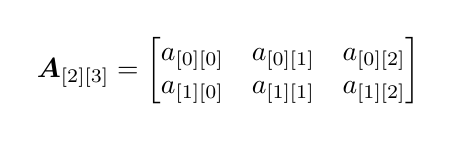
\begin{tikzpicture}[node distance = 0.5cm]
			% 绘制数组的数学表示
			\node (mathform) {
				\( \boldsymbol{A}_{[2][3]} = \begin{bmatrix}
					a_{[0][0]} & a_{[0][1]} & a_{[0][2]} \\
					a_{[1][0]} & a_{[1][1]} & a_{[1][2]} \\
				\end{bmatrix} \)
			};
			
			
		\end{tikzpicture}
	\end{center}
	
	\begin{figure}[h]
		\centering
		\centering
		\label{fig:t}
		\includegraphics[width=0.4\textwidth]{0220.png}
	\end{figure}
	
	
	当以列优先方式存储时,得出存储结构关系式为  
	
	\[ \text{LOC}(a_{i,j}) = \text{LOC}(a_{0,0}) + \big[j \times (h_1 + 1) + i\big] \times L \]  
	
	
	例如,对于数组 \( \boldsymbol{A}_{[2][3]} \),它按列优先方式在内存中的存储形式如图 3.19 所示。
	
	% 用tikz绘制二维数组按列优先存储的示意图
	\begin{center}
		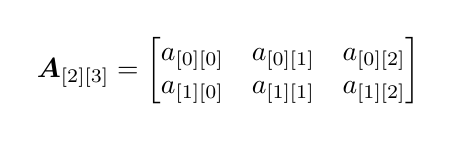
\begin{tikzpicture}[node distance = 0.5cm]
			% 绘制数组的数学表示
			\node (mathform) {
				\( \boldsymbol{A}_{[2][3]} = \begin{bmatrix}
					a_{[0][0]} & a_{[0][1]} & a_{[0][2]} \\
					a_{[1][0]} & a_{[1][1]} & a_{[1][2]} \\
				\end{bmatrix} \)
			};
			
		\end{tikzpicture}
	\end{center}
	
	\begin{figure}[h]
		\centering
		\centering
		\label{fig:t}
		\includegraphics[width=0.4\textwidth]{1148.png}
	\end{figure}
	
	若对一个 \( n \) 阶矩阵 \( \boldsymbol{A} \) 中的任意一个元素 \( a_{i,j} \) 都有 \( a_{i,j} = a_{j,i} \, (1 \leq i, j \leq n) \),则称其为对称矩阵。其中的元素可以划分为 3 个部分,即上三角区、主对角线和下三角区,如图 3.20 所示。
	
	\begin{figure}[h]
		\centering
		\centering
		\label{fig:t}
		\includegraphics[width=0.3\textwidth]{1257.png}
	\end{figure}
	
	对于 \( n \) 阶对称矩阵,上三角区的所有元素和下三角区的对应元素相同,若仍采用二维数组存放,则会浪费几乎一半的空间,为此将 \( n \) 阶对称矩阵 \( \boldsymbol{A} \) 存放在一维数组 \( \text{B}[n(n + 1) / 2] \) 中,即元素 \( a_{i,j} \) 存放在 \( b_k \) 中。比如只存放下三角部分(含主对角线)的元素。
	
	
	在数组 \( \text{B} \) 中,位于元素 \( a_{i,j} \, (i \geq j) \) 前面的元素个数为:
	\begin{itemize}
		\item 第 1 行:1 个元素(\( a_{1,1} \))。
		\item 第 2 行:2 个元素(\( a_{2,1}, a_{2,2} \))。
		\item \(\cdots\cdots\)
		\item 第 \( i - 1 \) 行:\( i - 1 \) 个元素(\( a_{i-1,1}, a_{i-1,2}, \cdots, a_{i-1,i-1} \))。
		\item 第 \( i \) 行:\( j - 1 \) 个元素(\( a_{i,1}, a_{i,2}, \cdots, a_{i,j-1} \))。
	\end{itemize}
	
	因此,元素 \( a_{i,j} \) 在数组 \( \text{B} \) 中的下标 \( k = 1 + 2 + \cdots + (i - 1) + j - 1 = \frac{i(i - 1)}{2} + j - 1 \)(数组下标从 0 开始)。因此,元素下标之间的对应关系如下:  
	\[
	k = 
	\begin{cases} 
		\displaystyle \frac{i(i - 1)}{2} + j - 1, & i \geq j \, (\text{下三角区和主对角线元素}) \\[6pt]
		\displaystyle \frac{j(j - 1)}{2} + i - 1, & i < j \, (\text{上三角区元素} \, a_{i,j} = a_{j,i}) 
	\end{cases}
	\]  
	
	
	当数组下标从 1 开始时,可以采用同样的推导方法,请读者自行思考。
	
	
	\subsubsection{三角矩阵}
	下三角矩阵[见图 3.22(a)]中,上三角区的所有元素均为同一常量。其存储思想与对称矩阵类似,不同之处在于存储完下三角区和主对角线上的元素之后,紧接着存储对角线上方的常量一次,所以可以将 \( n \) 阶下三角矩阵 \( \boldsymbol{A} \) 压缩存储在 \( \text{B}[n(n + 1) / 2 + 1] \) 中。
	 
	元素下标之间的对应关系为  
	\[
	k = 
	\begin{cases} 
		\displaystyle \frac{i(i - 1)}{2} + j - 1, & i \geq j \, (\text{下三角区和主对角线元素}) \\[6pt]
		\displaystyle \frac{n(n + 1)}{2}, & i < j \, (\text{上三角区元素}) 
	\end{cases}
	\]  
	
	
	下三角矩阵在内存中的压缩存储形式如图 3.21 所示。
	
	\begin{figure}[h]
		\centering
		\centering
		\label{fig:tt}
		\includegraphics[width=0.35\textwidth]{1804.png}
	\end{figure}
	
	上三角矩阵[见图 3.22(b)]中,下三角区的所有元素均为同一常量。只需存储主对角线、上三角区上的元素和下三角区的常量一次,可将其压缩存储在 \( \text{B}[n(n + 1) / 2 + 1] \) 中。
	
	\begin{figure}[h]
		\centering
		\centering
		\label{fig:ttt}
		\includegraphics[width=0.35\textwidth]{1855.png}
	\end{figure}
	
	在数组 \( \text{B} \) 中,位于元素 \( a_{i,j} \, (i \leq j) \) 前面的元素个数为:
	\begin{itemize}
		\item 第 1 行:\( n \) 个元素  
		\item 第 2 行:\( n - 1 \) 个元素  
		\item \(\cdots\cdots\)  
		\item 第 \( i - 1 \) 行:\( n - i + 2 \) 个元素  
		\item 第 \( i \) 行:\( j - i \) 个元素  
	\end{itemize}
	
	因此,元素 \( a_{i,j} \) 在数组 \( \text{B} \) 中的下标  
	\[
	k = n + (n - 1) + \cdots + (n - i + 2) + (j - i + 1) - 1 = \frac{(i - 1)(2n - i + 2)}{2} + (j - i)
	\]  
	
	因此,元素下标之间的对应关系如下:  
	\[
	k = 
	\begin{cases} 
		\displaystyle \frac{(i - 1)(2n - i + 2)}{2} + (j - i), & i \leq j \, (\text{上三角区和主对角线元素}) \\[6pt]
		\displaystyle \frac{n(n + 1)}{2}, & i > j \, (\text{下三角区元素}) 
	\end{cases}
	\]  
	
	
	\subsubsection{三对角矩阵}
	对角矩阵也称带状矩阵。对 \( n \) 阶矩阵 \( \boldsymbol{A} \) 中的任意一个元素 \( a_{i,j} \),当 \( |i - j| > 1 \) 时,若有 \( a_{i,j} = 0 \, (1 \leq i, j \leq n) \),则称为三对角矩阵,如图 3.24 所示。在三对角矩阵中,所有非零元素都集中在以主对角线为中心的 3 条对角线的区域,其他区域的元素都为零。
	
	
	三对角矩阵 \( \boldsymbol{A} \) 也可以采用压缩存储,将 3 条对角线上的元素按行优先方式存放在一维数组 \( \text{B} \) 中,且 \( a_{1,1} \) 存放于 \( \text{B}[0] \) 中,其存储形式如图 3.25 所示。
	

	
	
	由此可以计算矩阵 \( \boldsymbol{A} \) 中 3 条对角线上的元素 \( a_{i,j} \, (1 \leq i, j \leq n, \, |i - j| \leq 1) \) 在一维数组 \( \text{B} \) 中存放的下标为 \( k = 2i + j - 3 \)。  
	
	
	反之,若已知三对角矩阵中的某个元素 \( a_{i,j} \) 存放在一维数组 \( \text{B} \) 的第 \( k \) 个位置,则有 \( i = \lfloor (k + 1) / 3 \rfloor + 1 \),\( j = k - 2i + 3 \)。例如,当 \( k = 0 \) 时,\( i = \lfloor (0 + 1) / 3 \rfloor + 1 = 1 \),\( j = 0 - 2 \times 1 + 3 = 1 \),存放的是 \( a_{1,1} \);当 \( k = 2 \) 时,\( i = \lfloor (2 + 1) / 3 \rfloor + 1 = 2 \),\( j = 2 - 2 \times 2 + 3 = 1 \),存放的是 \( a_{2,1} \);当 \( k = 4 \) 时,\( i = \lfloor (4 + 1) / 3 \rfloor + 1 = 2 \),\( j = 4 - 2 \times 2 + 3 = 3 \),存放的是 \( a_{2,3} \)。  
	
	
	\paragraph{next 数组和 PM 表的关系}
	next 数组和 PM 表的关系是怎样的?  
	
	通过上述举例,可以推理出 next 数组和 PM 表之间的关系:  
	\[
	\begin{aligned}
		\text{next}[j] &= j - \text{右滑位数} = j - \big( \text{已匹配的字符数}^{\textcircled{1}} - \text{对应的部分匹配值} \big) \\
		&= j - \big[ (j - 1) - \text{PM}[j - 1] \big] \\
		&= \text{PM}[j - 1] + 1
	\end{aligned}
	\]  
	
	
	\subsubsection{*next 数组的推理公式}
	如何推理 next 数组的一般公式?设主串为 \( 's_1 s_2 \cdots s_n' \),模式串为 \( 'p_1 p_2 \cdots p_m' \),当主串的第 \( i \) 个字符与模式串的第 \( j \) 个字符失配时,应让主串当前位置与模式串的哪个字符进行比较?  
	
	假设此时应与模式串的第 \( k \, (k < j) \) 个字符进行比较,则模式串的前 \( k - 1 \) 个字符的子串必须满足下列条件,且不可能存在 \( k' > k \) 满足下列条件:  
	\[ 'p_1 p_2 \cdots p_{k-1}' = 'p_{j-k+1} p_{j-k+2} \cdots p_{j-1}' \]  
	
	
	若存在满足如上条件的子串,则发生失配时,仅需将模式串的第 \( k \) 个字符和主串的第 \( i \) 个字符对齐,此时模式串的前 \( k - 1 \) 个字符的子串必定与主串的第 \( i \) 个字符之前长度为 \( k - 1 \) 的子串相等,因此,只需从模式串的第 \( k \) 个字符与主串的第 \( i \) 个字符进行比较即可,如图 4.3 所示。
	
	% 用tikz绘制模式串右滑示意图
	
	
	
	当模式串已匹配相等序列中不存在满足上述条件的子串时(可视为 \( k = 1 \)),显然应让主串的第 \( i \) 个字符和模式串的第 1 个字符进行比较。  
	
	当模式串的第 1 个字符(\( j = 1 \))与主串的第 \( i \) 个字符发生失配时,规定 \( \text{next}[1] = 0 \)。  
	
	
	通过上述分析可以得出 next 函数的公式:  
	\[
	\text{next}[j] = 
	\begin{cases} 
		0, & j = 1 \\[4pt]
		\max\big\{ k \mid 1 < k < j \text{ 且 } 'p_1 \cdots p_{k-1}' = 'p_{j-k+1} \cdots p_{j-1}' \big\}, & \text{当此集合不为空时} \\[4pt]
		1, & \text{其他情况} 
	\end{cases}
	\]  
	
	
	要用代码来实现,难度貌似还不小,下面来尝试推理求解的科学步骤。  
	
	首先由公式可知  
	\[ \text{next}[1] = 0 \]  
	
	设 \( \text{next}[j] = k \),此时 \( k \) 应满足的条件在上文中已描述。  
	
	此时 \( \text{next}[j + 1] = ? \) 可能有两种情况:  
	
	\begin{enumerate}
		\item 若 \( p_k = p_j \),则表明在模式串中  
		\[ 'p_1 \cdots p_{k-1} p_k' = 'p_{j-k+1} \cdots p_{j-1} p_j' \]  
		% 后续若有内容可继续补充
	\end{enumerate}  
	
	% 后续若有内容可继续补充
	% 后续若有内容可继续补
	
\end{document}